\documentclass{beamer}
\usetheme[pageofpages=of,% String used between the current page and the
                         % total page count.
          bullet=circle,% Use circles instead of squares for bullets.
          titleline=true,% Show a line below the frame title.
          alternativetitlepage=true,% Use the fancy title page.
       %   titlepagelogo=logo-polito,% Logo for the first page.
       %   watermark=watermark-polito,% Watermark used in every page.
       %   watermarkheight=100px,% Height of the watermark.
       %   watermarkheightmult=4,% The watermark image is 4 times bigger
                                % than watermarkheight.
          ]{Torino}

\setbeamertemplate{footline}{
  \begin{beamercolorbox}[wd=\paperwidth,ht=1ex,dp=1ex]{footline}
    \vspace{5pt} \hspace{1em} \insertframenumber/\inserttotalframenumber
  \end{beamercolorbox}
}

\newcommand{\given}{\,|\,}

\usepackage{colortbl}
\definecolor{LightGray}{gray}{0.9}
\definecolor{DarkGray}{gray}{0.3}
\definecolor{LightCyan}{rgb}{0.9, 1, 1}
\definecolor{LightRed}{rgb}{1, 0.8, 0.8}
\definecolor{LightGreen}{rgb}{0.8, 1, 0.8}
\definecolor{DarkGreen}{rgb}{0.3, 0.5, 0.3}



\author{Brendon J. Brewer}
\title{Introduction to Bayesian Statistics}
\institute{Summer Institute in Statistical Genomics \\
The University of Auckland, November 2026}
\date{}


\linespread{1.3}
\usepackage{minted}
\usepackage[utf8]{inputenc}
\usepackage{dsfont}


\begin{document}

\frame{\titlepage}

\begin{frame}
\frametitle{About Me}

\url{https://brendonbrewer.com/}
\pause

\begin{itemize}
\item I have a background in astrophysics and am currently a senior lecturer
in statistics. Bayesian inference is my main area. \pause
\item However, I am definitely not in genomics.
\end{itemize}


\end{frame}



\begin{frame}
\frametitle{Probability as Plausibility}
The main distinction between Bayesian and frequentist/classical statistics
is the meaning of probability. What we think a probability {\em is}
influences {\em what calculations we think it is valid to do.}\\[0.5em]\pause

In Bayesian statistics, $P(A \given B)$ means how plausible statement $A$ is,
assuming that $B$ is true (this might be hypothetical --- {\em if} $B$
were true --- or we might actually know $B$ is true).

\end{frame}



\begin{frame}
\frametitle{Example of Probability as Plausibility}
Suppose there is some {\bf statement}
or {\bf proposition} $A$, and we are not sure whether it is true or
false. For example, {\em $A \equiv$ New Zealand wins more bronze medals than
Australia at the 2028 Olympics}.\pause

We can describe the degree of plausibility of $A$ using a value between 0 and 1.
For instance:
\begin{itemize}
\item $P(A) = 1$ (it is definitely true) \\
\item $P(A) = 0$ (it is definitely false) \\
\item $P(A) = 0.1$ (it is probably false) \\
\item $P(A) = 0.5$ (as certain as a coin landing heads)
\end{itemize}

\end{frame}


\begin{frame}
\frametitle{Bayesian Interpretations of Probability}
There are some language choices people use to describe what
Bayesian probabilities represent. Examples:\pause

\begin{itemize}
\item Plausibility \pause
\item Degree of confidence \pause
\item Degree of belief \pause
\item The degree to which one statement implies another
\end{itemize}

\end{frame}



\begin{frame}
\frametitle{Subjective Probabilities}
Some people say that Bayesian probabilities are subjective.
This is often true. It is certainly the case
that they depend on what information you have.\\[0.3em]\pause

Consider the statement that NZ's population is greater than 8
million people. I would assign a probability close to zero.
Someone from afar might assign a probability closer to 0.5.\\[0.3em]\pause

When different people have different probability judgments,
it is usually because they have different information or assumptions.

\end{frame}


\begin{frame}
\frametitle{Assumptions}
\begin{itemize}
\item Even though different people might have different probability
judgments, the rules linking one probability to another --- the sum
and product rule (etc) --- are consistent.\\\pause
\item When we start working on problems, we will see that some
input probabilities in the problem
are judgment calls, but other ones are calculated.\\\pause
\item The most obvious place where assumptions are needed is the
`prior' which we will meet soon, but it's not the only place
where assumptions enter.
\end{itemize}

\end{frame}


\begin{frame}
\frametitle{Updating Probabilities}
There is a well-defined procedure for updating probabilities to take new
information into account. For example, suppose you are interested in
the proposition $A$.\pause
\begin{itemize}
\item You assign a {\bf prior} probability $P(A)$.\pause
\item Then, you learn that
some related proposition $B$ is true. You should update your probability
to $P(A \given B)$, called a {\bf posterior} probability.\pause
\item If you then learn that $C$ is true, you should update
to $P(A \given B, C)$, another posterior probability.\pause
\item And so on.
\end{itemize}

\end{frame}



\begin{frame}
\frametitle{Updating Probabilities: Bayes' Rule}
Bayes' rule (derived from the product rule) gives us the procedure to
calculate updated (posterior) probabilities.

\begin{align}
P(H \given D) &= \frac{P(H) P(D\given H)}{P(D)}.
\end{align}

\pause
The terms have names:
\begin{align}
\textnormal{posterior prob.} &=
        \frac{\textnormal{prior prob.} \times \textnormal{likelihood}}{\textnormal{marginal likelihood}}
\end{align}

\end{frame}



\begin{frame}
\frametitle{Updating Probabilities: Bayes' Rule}
The statements in the previous equation were $H$ and $D$.
These stand for {\em hypothesis} and {\em data} respectively,
to indicate how we use Bayes' theorem.\\[0.5em]\pause

We usually want to know if $H$ is true, and we don't know,
so we calculate a probability for it. We usually have some
data proposition $D$ which we do know is true, so we use that.

\end{frame}


\begin{frame}
\frametitle{Interpretation of the Terms}

\begin{itemize}
\item $P(H\given D)$ is the updated (posterior) probability, which we
want.\pause
\item $P(H)$ is the initial (prior) probability. It describes
how plausible $H$ is without taking $D$ into account.\pause
\item $P(D \given H)$ is the likelihood value --- how plausible would $D$
have been if we knew $H$ was true?\pause
\item $P(D)$ is the marginal likelihood\footnote{Sometimes called the
{\bf evidence}, especially by physicists.} --- how plausible would $D$ have been
whether $H$ is true or not?
\end{itemize}

\end{frame}


\begin{frame}
\frametitle{Input and Output}
Two of the probabilities --- the prior and the likelihood --- are inputs to
the calculation, that we assign based on judgment calls or prior/external
information.\\

The other two --- the posterior and the marginal likelihood --- are outputs
that we compute.
\end{frame}


\begin{frame}
\frametitle{More Than One Hypothesis}
Usually there is more than one hypothesis of interest, so we will calculate
more than one posterior probability. For example, $P(H_1 \given D)$ and
$P(H_2 \given D)$. In fact, for any $H$, the negation $\neg H$ exists
(it means {\bf $H$ is false}), so there are always at least two hypotheses.


\end{frame}


\begin{frame}
\frametitle{First Example}
\begin{itemize}
\item There are two balls in a bag \pause
\item We don't know which of the following possibilities is true:\\\pause
{\em $BB$: Both balls are black}\\
{\em $BW$: One is black and one is white}
\end{itemize}\pause

Note: $BW = \neg BB$.
\end{frame}


\begin{frame}
\frametitle{Data}
To help us figure out which hypothesis is true, one ball is picked
from the bag. {\bf It is black}. What happens to the plausibility of
the hypothesis $BB$, that both are black?\pause

\begin{itemize}
\item[(a)] It is now more plausible
\item[(b)] It is now less plausible
\item[(c)] No change.
\end{itemize}\pause

I hope your intuition chooses (a). We will now do the calculation to
show exactly how plausible $BB$ is.


\end{frame}


\begin{frame}
\frametitle{Bayes Box}
In the first part of the course, we will make tables of probabilities
which we call a Bayes Box. It gives a simple view of the probabilities
involved in the problem.\\[0.5em]\pause

\begin{tabular}{|c|c|c|c|c|}
\hline
Hypothesis & Prior & Likelihood & Prior $\times$ Likelihood & Posterior \\
\hline
$BB$ & 0.5 & & & \\
$BW$ & 0.5 & & & \\
\hline
Total & 1 & & & \\
\hline
\end{tabular}

\end{frame}


\begin{frame}
\frametitle{Prior Probabilities}
In the Bayes Box on the previous slide, I have assigned uniform (equal)
prior probabilities of 0.5 to the two hypotheses. This represents the state
of having no idea apart from the fact that there are two possibilities.\pause

\begin{alertblock}{Note}
The sum of the values in the prior column should always be 1.
The prior column forms a discrete probability distribution.
We sometimes just call it ``the prior distribution'' or just ``the prior''.
\end{alertblock}


\end{frame}



\begin{frame}
\frametitle{Bar Plot of the Prior Probabilities}

\centering
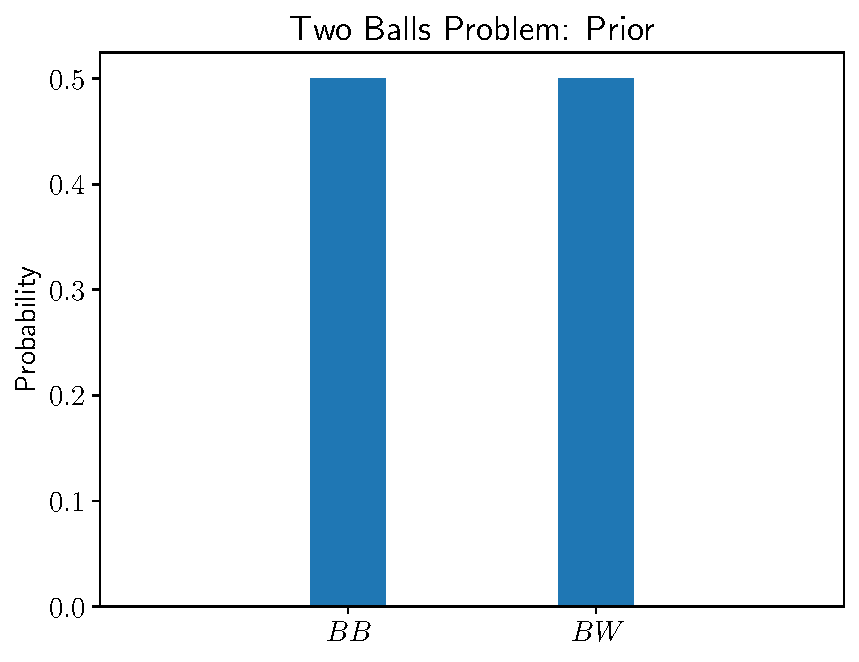
\includegraphics[width=0.7\textwidth]{images/two_balls_prior.pdf}

\end{frame}



\begin{frame}
\frametitle{More Input Needed}
To compute the posterior probabilities (which we want to do), we need
the likelihood values. These represent the probability of the data, assuming
each hypothesis is true (hypothetically), in turn. The data was
$D = $~{\bf black ball was drawn}.\pause

The values are:
\begin{align}
P(D \given BB) &= 1 \\
P(D \given BW) &= 0.5
\end{align}
Why? {\bf Imagine knowing the answer, but not knowing the data.}

\end{frame}

\begin{frame}
\frametitle{Bayes Box}
We now have more values for our Bayes Box.\\[0.5em]\pause
\begin{tabular}{|c|c|c|c|c|}
\hline
Hypothesis & Prior & Likelihood & Prior $\times$ Likelihood & Posterior \\
\hline
$BB$ & 0.5 & 1 & & \\
$BW$ & 0.5 & 0.5 & & \\
\hline
Total & 1 & & & \\
\hline
\end{tabular}\pause

\begin{alertblock}{Likelihoods}
We call this column the ``likelihood function'' or just ``the likelihood''.
The sum does not need to be 1, and is meaningless in
general.
\end{alertblock}

\end{frame}


\begin{frame}
\frametitle{Bayes Box}
The rest of the Bayes Box is not {\em assigned}, but is {\em computed}
using the rules of probability theory. Specifically, Bayes' rule applied
twice: once to get $P(BB \given D)$ and once to get $P(BW \given D)$.
It is easy to do the calculation using the Bayes Box. First just multiply
priors by likelihoods, then sum the column:
\\[0.5em]\pause
\begin{tabular}{|c|c|c|c|c|}
\hline
Hypothesis & Prior & Likelihood & Prior $\times$ Likelihood & Posterior \\
\hline
$BB$ & 0.5 & 1 & 0.5 & \\
$BW$ & 0.5 & 0.5 & 0.25 & \\
\hline
Total & 1 & & 0.75 & \\
\hline
\end{tabular}\pause



\end{frame}


\begin{frame}
\frametitle{Bayes Box}
We almost have the result! The priors times the likelihoods gives us the
{\em relative} updated plausibility of the two hypotheses. To become a
probability distribution, we need to force it to sum to 1. We do this
using ``normalisation'', i.e., dividing the column by its own total:\\[0.5em]\pause
\begin{tabular}{|c|c|c|c|c|}
\hline
Hypothesis & Prior & Likelihood & Prior $\times$ Likelihood & Posterior \\
\hline
$BB$ & 0.5 & 1 & 0.5 & 2/3 \\
$BW$ & 0.5 & 0.5 & 0.25 & 1/3 \\
\hline
Total & 1 & & 0.75 & 1\\
\hline
\end{tabular}\pause



\end{frame}


\begin{frame}
\frametitle{Marginal Likelihood}
The sum of the prior times likelihood column is the marginal likelihood
or evidence $P(D)$. It has two uses --- one of which we just saw.\\[0.5em]\pause

We can understand it as being the sum of the two mutually exclusive ways
$D$ could have come true --- via $BB$ or via $BW$. Mathematically this is
the {\bf partition theorem} which you might have seen before:
\begin{align}
P(D) &= P(BB)P(D \given BB) + P(BW)P(D \given BW).
\end{align}
\pause
More generally,
\begin{align}
P(D) &= \sum_i P(H_i, D) = \sum_i P(H_i)P(D \given H_i).
\end{align}

\end{frame}


\begin{frame}
\frametitle{Posterior Probabilities}
The posterior probabilities now add up to 1 and form the posterior distribution,
or just ``the posterior''. We see that the probabilities have changed from
50:50 to 67:33 based on the data.\pause

\begin{alertblock}{Outputs}
The posterior distribution and the marginal likelihood are the outputs of the
calculation.
\end{alertblock}

\end{frame}

\begin{frame}
\frametitle{Bar Plot of the Posterior Probabilities}

\centering
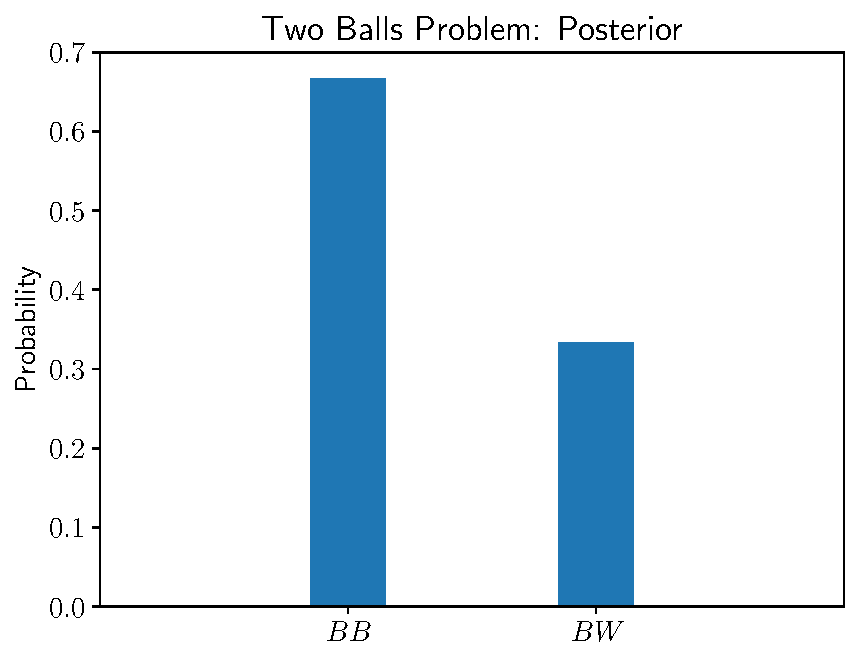
\includegraphics[width=0.7\textwidth]{images/two_balls_posterior.pdf}

\end{frame}


\begin{frame}[fragile]
\frametitle{R Code for Bayes Box Calculation}
The calculation equivalent to a Bayes Box (or Bayes' rule twice) can be
done easily in R. Each column of the Bayes Box is an R {\bf vector}.\pause

\begin{minted}{r}
prior = rep(0.5, 2)
lik = c(1, 0.5)
h = prior*lik
Z = sum(h)
post = h/Z
\end{minted}
\pause
For some reason, \mintinline{r}{h} is the traditional symbol for prior times
likelihood, and \mintinline{r}{Z} for the marginal likelihood.
\end{frame}

\begin{frame}
\frametitle{More Data}
What happens if we accumulate more data? Suppose the experiment was repeated
a further 4 times (so 5 in total), and the outcome was the same every time,
i.e., {\bf the black ball was drawn five times}. This seems like compelling
evidence for $BB$ and against $BW$. What are the posterior probabilities?

\end{frame}

\begin{frame}
\frametitle{More Data}
Let's go back to our 50/50 prior, and consider the data
proposition $D_5 = $~the black ball was drawn five times.
We need likelihood values.\pause

If $BB$ is true, what is the probability of $D_5$?
\begin{align}
P(D_5 \given BB) &= 1.
\end{align}
\pause
If $BW$ is true, what is the probability of $D_5$?
\begin{align}
P(D_5 \given BW) &= \frac{1}{2}\times\frac{1}{2}\times\frac{1}{2}\times
                    \frac{1}{2}\times\frac{1}{2}\\
                 &= \frac{1}{32}.
\end{align}\pause
When there is more than one data point, the likelihood is a
product.

\end{frame}


\begin{frame}
\frametitle{Filling in the Bayes Box}
\begin{tabular}{|c|c|c|c|c|}
\hline
Hypothesis & Prior & Likelihood & Prior $\times$ Likelihood & Posterior \\
\hline
$BB$ & 0.5 & 1 & 0.5 & 0.9696... \\
$BW$ & 0.5 & 0.03125 & 0.015625 & 0.0303... \\
\hline
Total & 1 & & 0.515625 & 1\\
\hline
\end{tabular}
\pause

$BB$ is now highly plausible and $BW$ is quite implausible.

\end{frame}



\begin{frame}
\frametitle{Sequential Updating}

\begin{itemize}
\item To solve the inference with the ``5 black draws'' example,
we went back to the beginning, back to a 50/50 prior and
using the likelihood for 5 black draws\pause
\item Instead, we could have started with the 67/33 prior and then used
the likelihood for 4 extra black draws\pause
\item  The answers would have been the same, but usually
``back to the beginning'' is more convenient\pause
\item If done sequentially, 
the posterior after analysing one data set becomes
the prior for analysing the next.
\end{itemize}


\end{frame}

\begin{frame}
\frametitle{Sequential Updating}
We can watch the posterior change, assuming the black ball continues to be
drawn. If the white ball were ever drawn, the posterior would ``snap'' to $BW$.

\centering
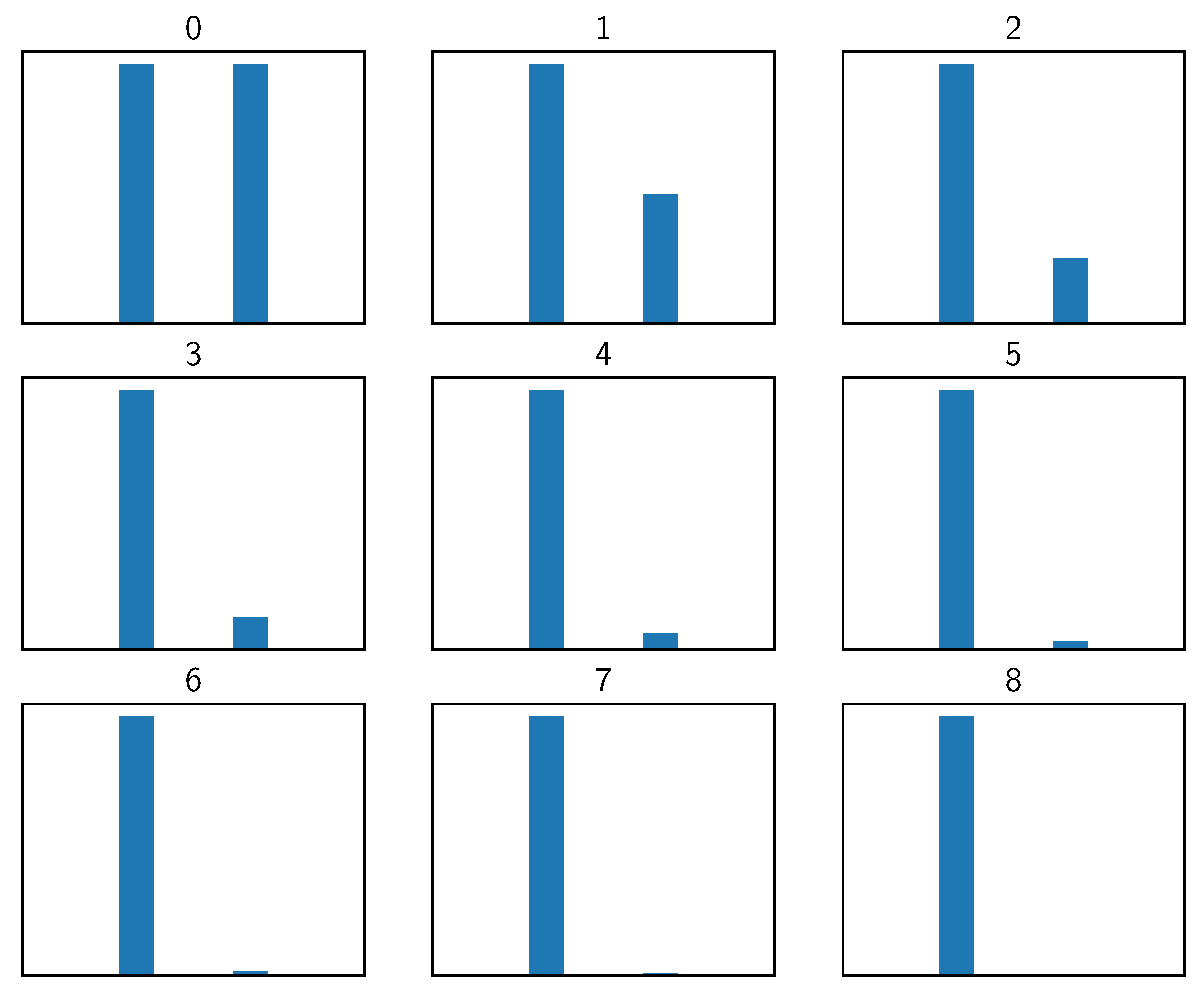
\includegraphics[width=0.4\textwidth]{images/two_balls_updating.pdf}

\end{frame}


\begin{frame}
\frametitle{Sequential Updating}
We can watch the posterior change, assuming the black ball continues to be
drawn. If the white ball were ever drawn, the posterior would ``snap'' to $BW$.

\centering
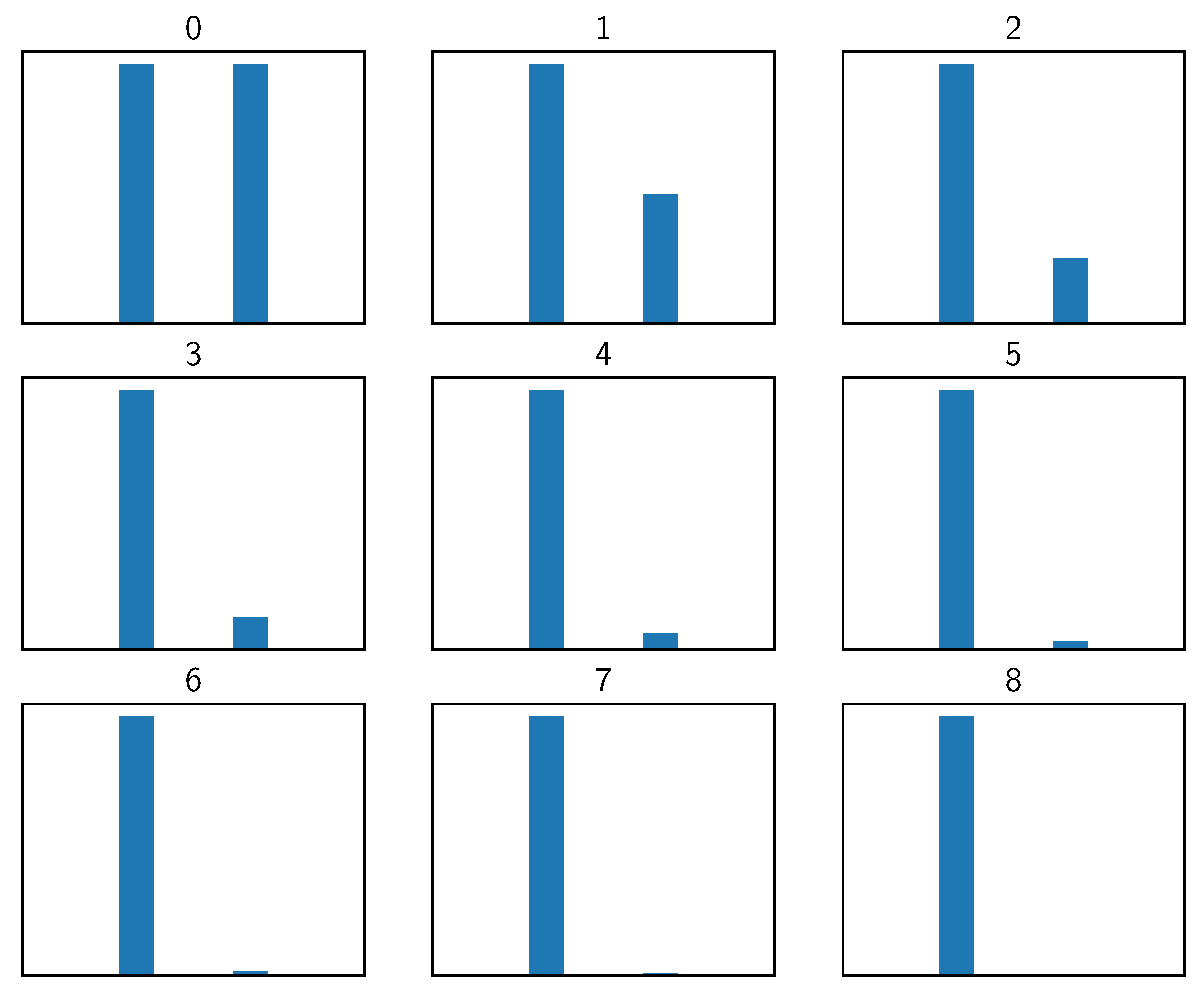
\includegraphics[width=0.4\textwidth]{images/two_balls_updating.pdf}

\end{frame}



\begin{frame}
\frametitle{Different Priors}
Suppose we didn't start with a 50/50 prior, but were initially sceptical of
$BB$ for some reason, giving it a prior probability of 0.01.
We would have to give $BW$ a prior probability of 0.99.

\end{frame}

\begin{frame}
\frametitle{Bayes Box, Sceptical Prior}
\begin{tabular}{|c|c|c|c|c|}
\hline
Hypothesis & Prior & Likelihood & Prior $\times$ Likelihood & Posterior \\
\hline
$BB$ & 0.01 & 1 & 0.01 & 0.2443 \\
$BW$ & 0.99 & 0.03125 & 0.0309375 & 0.7557 \\
\hline
Total & 1 & & 0.0409375 & 1\\
\hline
\end{tabular}
\pause
\\[0.5em]
The data has made $BB$ more plausible than it was before, but we are not yet
convinced of it.


\end{frame}


\begin{frame}
\frametitle{Different Priors}
If we start with a low prior probability for one of the hypotheses, it takes
{\bf more data} to increase the probability to a high level.



    \begin{columns} % Create two columns
        \column{0.5\textwidth} % Left column (50% width)
        \hspace{2em}
        
\includegraphics[width=0.6\linewidth]{images/sagan.jpg}

        \column{0.5\textwidth} % Right column (50% width)
        ``Extraordinary claims require extraordinary evidence'' --
        Carl Sagan (image credit: NASA/JPL)
     \end{columns}


\end{frame}

\begin{frame}
\frametitle{Different Data}
If we ever drew the white ball from the bag, we would immediately become
100\% certain of $BW$. What in Bayes' rule (or a Bayes Box) would cause this
to happen?

\end{frame}


\begin{frame}
\frametitle{An Extreme Prior}
\begin{itemize}
\item What if we start with this extreme prior?
\begin{align}
P(BB) &= 0 \\
P(BW) &= 1.
\end{align}

\item What would be the posterior probability of $BB$ after drawing the black
ball 1 million times?

\end{itemize}

\end{frame}



\begin{frame}
\frametitle{Cromwell's Rule}

{\em ``I beseech you, in the bowels of Christ, think it possible that
you may be mistaken.''} - Oliver Cromwell \\[1em]\pause

{\em ``Leave a little probability for the moon being made of green
cheese; it can be as small as 1 in a million, but have it
there since otherwise an army of astronauts returning
with samples of the said cheese will leave you unmoved.''}
- Dennis Lindley

\end{frame}


\begin{frame}
\frametitle{Product Space View I}
There is another way of looking at the Bayesian update, which I call the
{\bf product space view} (not standard terminology).
We will consider the data $D$ and also the alternative value for the data
$\neg D$. We can create a 2$\times$2 grid of the {\bf joint
prior} distribution. The marginal for the hypothesis is the prior,
and the marginal for the data is called the `prior predictive
distribution'.
\begin{center}
\begin{tabular}{|c|cc|c|}
\hline
   &  $BB$ &  $BW$ & Marginal for data\\
\hline
%\rowcolor{LightGreen}
Black ball ($D$)      &  $1/2$  &  $1/4$     & $3/4$\\
%\rowcolor{LightRed}
White ball ($\neg D$) &  0      &  $1/4$     & $1/4$\\
\hline
Marginal for hypotheses   &  $1/2$  & $1/2$  & 1\\
\hline
\end{tabular}
\end{center}

\end{frame}

\begin{frame}
\frametitle{Product Space View II}
The values for the joint probabilities are obtained by using
prior probabilities (e.g., $P(BW)$) multiplied by
probabilities about the data (e.g., $P(D \given BW)$) using the product
rule. E.g.:
\begin{align}
P(BW, D) &= P(BW)P(D \given BW) = 1/2 \times 1/2 = 1/4.
\end{align}

\pause

Probability distributions for the data {\em given the hypotheses} are
traditionally called sampling distributions, but really they are
a type of prior.

\end{frame}



\begin{frame}
\frametitle{Product Space View III}
The Bayesian update involves simply deleting/setting to zero
all the possibilities that are now false, and renormalising the
result using the marginal likelihood, which is just one of the
probabilities from the prior predictive distribution.
\begin{center}
\begin{tabular}{|c|cc|c|}
\hline
   &  $BB$ &  $BW$ & Marginal for data\\
\hline
%\rowcolor{LightGreen}
Black ball ($D$)      &  $1/2$  &  $1/4$     & $3/4$\\
\rowcolor{LightRed}
White ball ($\neg D$) &  0      &  0     & 0 \\
\hline
Marginal for hypotheses  &  $1/2$  & $1/2$  & 1\\
\hline
\end{tabular}
\end{center}

\end{frame}

\begin{frame}
\frametitle{Product Space View IV}
\begin{center}
\begin{tabular}{|c|cc|c|}
\hline
   &  $BB$ &  $BW$ & Marginal for data\\
\hline
\rowcolor{LightGreen}
Black ball ($D$)      &  $2/3$  &  $1/3$     & $1$\\
\rowcolor{LightRed}
White ball ($\neg D$) &  0      &  0     & 0 \\
\hline
Marginal for hypotheses  &  $2/3$  & $1/3$  & 1\\
\hline
\end{tabular}
\end{center}

\pause
The product space view is very useful for thinking about
what it is that we are doing. It is less useful for actually
doing calculations --- for that we'll usually stick to the Bayes'
Box.
\end{frame}


\begin{frame}
\frametitle{Bayes' Rule for Sets of Hypotheses}
Suppose we have a set of mutually exclusive and exhaustive hypotheses
$H_1, ..., H_n$. This means one and only one of them is true --- this is usually
the way things are initially arranged and the medical testing example was an
exception.\pause

Bayes' rule for the posterior probability of each hypothesis $H_i$:
\begin{align}
P(H_i \given D) &= \frac{P(H_i)P(D \given H_i)}{P(D)}
\end{align}\pause
The marginal likelihood involves a sum over all hypotheses:
\begin{align}
P(D) &= \sum_{i=1}^n P(H_i)P(D \given H_i).
\end{align}

\end{frame}


\begin{frame}
\frametitle{Bayes' Rule $n$ times $\equiv$ Bayes Box}
Using a Bayes Box with $n$ rows and applying the procedure there
(once you have assigned priors and likelihoods) is equivalent
to using Bayes' rule $n$ times and the marginal likelihood formula
as given on the previous slide.

\end{frame}

\begin{frame}

\begin{center}
\Large
Parameter Estimation
\end{center}

\end{frame}


\begin{frame}
\frametitle{Parameter Estimation}

\begin{itemize}
\item Parameter estimation is a really important part of statistics.\pause
\item A parameter is {\bf a quantity whose value we would like to
        know.}\footnote{It's a bit more than this, but this will do for now.}\pause
\item We will describe our uncertainty about the value of the parameter
using a {\bf probability distribution}.\pause
\item This gets updated from a {\bf prior distribution}
    to a {\bf posterior distribution}
    as we get more information.
\end{itemize}

\end{frame}

\begin{frame}
\frametitle{Parameter Estimation}
Recall that Bayes' rule can be used on a set of mutually exclusive hypotheses.
These can be statements about the value of the parameter $\theta$.\pause

\begin{itemize}
\item One hypothesis might be ``$\theta = 1$'' \pause
\item Another might be ``$\theta = 2$'' \pause
\item We might get some data like ``$x = 3$''.
\end{itemize}

\end{frame}


\begin{frame}
\frametitle{Bayes' Rule Lots of Times}
\begin{align}
P(\theta = 1 \given x = 3) &= \frac{P(\theta=1)P(x=3 \given \theta=1)}{P(x=3)}\\
P(\theta = 2 \given x = 3) &= \frac{P(\theta=2)P(x=3 \given \theta=2)}{P(x=3)}\\
&...&\\
P(\theta = 9 \given x = 3) &= \frac{P(\theta=9)P(x=3 \given \theta=9)}{P(x=3)}\\
\end{align}

\end{frame}

\begin{frame}
\frametitle{Bayes' Rule Lots of Times}
\begin{align}
\color{red}{P(\theta = 1 \given x = 3)} &= \frac{{\color{blue}P(\theta=1)}P(x=3 \given \theta=1)}{P(x=3)}\\
\color{red}{P(\theta = 2 \given x = 3)} &= \frac{{\color{blue}P(\theta=2)}P(x=3 \given \theta=2)}{P(x=3)}\\
&...&\\
\color{red}{P(\theta = 9 \given x = 3)} &= \frac{{\color{blue}P(\theta=9)}P(x=3 \given \theta=9)}{P(x=3)}\\
\end{align}

{\color{red}Posterior Distribution}
{\color{blue}Prior Distribution}

\end{frame}


\begin{frame}
\frametitle{Bayes' Rule Lots of Times}
\begin{align}
P(\theta = 1 \given x = 3) &= \frac{P(\theta=1){\color{orange}P(x=3 \given \theta=1)}}{\color{green}P(x=3)}\\
P(\theta = 2 \given x = 3) &= \frac{P(\theta=2){\color{orange}P(x=3 \given \theta=2)}}{\color{green}P(x=3)}\\
&...&\\
P(\theta = 9 \given x = 3) &= \frac{P(\theta=9){\color{orange}P(x=3 \given \theta=9)}}{\color{green}P(x=3)}\\
\end{align}

{\color{orange}Likelihood Function}
{\color{green}Marginal Likelihood (common to all $\theta$ values)}

\end{frame}

\begin{frame}
\frametitle{Bayes Box for Parameter Estimation}
Since a Bayes Box is equivalent to these repeated uses of Bayes' rule,
we can use them for parameter estimation (when there is only one unknown
parameter).

\end{frame}


\begin{frame}
\frametitle{Example Bayes Box for Parameter Estimation}
\begin{tabular}{|c|c|c|c|c|}
\hline
Parameter & Prior & Likelihood & Prior $\times$ Likelihood & Posterior \\
$\theta$  & $p(\theta)$ & $p(x \given \theta)$ & $p(\theta)p(x\given\theta)$ & $p(\theta\given x)$ \\
\hline
0.1 & 0.2  &  & & \\
0.2 & 0.2  &  & & \\
0.3 & 0.2 &  & & \\
0.4 & 0.2  &  & & \\
0.5 & 0.2 & & & \\
\hline
Total & 1 & & & 1 \\
\hline
\end{tabular}
\pause
\vspace{1em}

Note the notation for the columns with the lower case $p$
which means ``probability distribution for''.


\end{frame}


\begin{frame}
\frametitle{Bayes' Rule for Parameter Estimation}
Instead of writing down Bayes' rule lots of times, we often write it down
once only, with each term being a whole function of $\theta$ not just
a single probability.\pause
\begin{align}
p(\theta \given x) &= \frac{p(\theta)p(x \given \theta)}{p(x)} \\
p(\theta \given x) &\propto p(\theta)p(x \given \theta) \\
\texttt{posterior} &\propto \texttt{prior} \times \texttt{likelihood}
\end{align}
\pause
(notation: $\theta$=parameter, $x$=data)
We will use this more when we do {\bf analytical methods}. For now, we will
stick to the Bayes Box.


\end{frame}


\begin{frame}
\frametitle{What Usually Happens}
Usually, the prior distribution $p(\theta)$ is something wide (indicating
a lot of uncertainty). After analysing data we get the posterior distribution
$p(\theta \given x)$ which is usually narrower than the prior.

\begin{center}
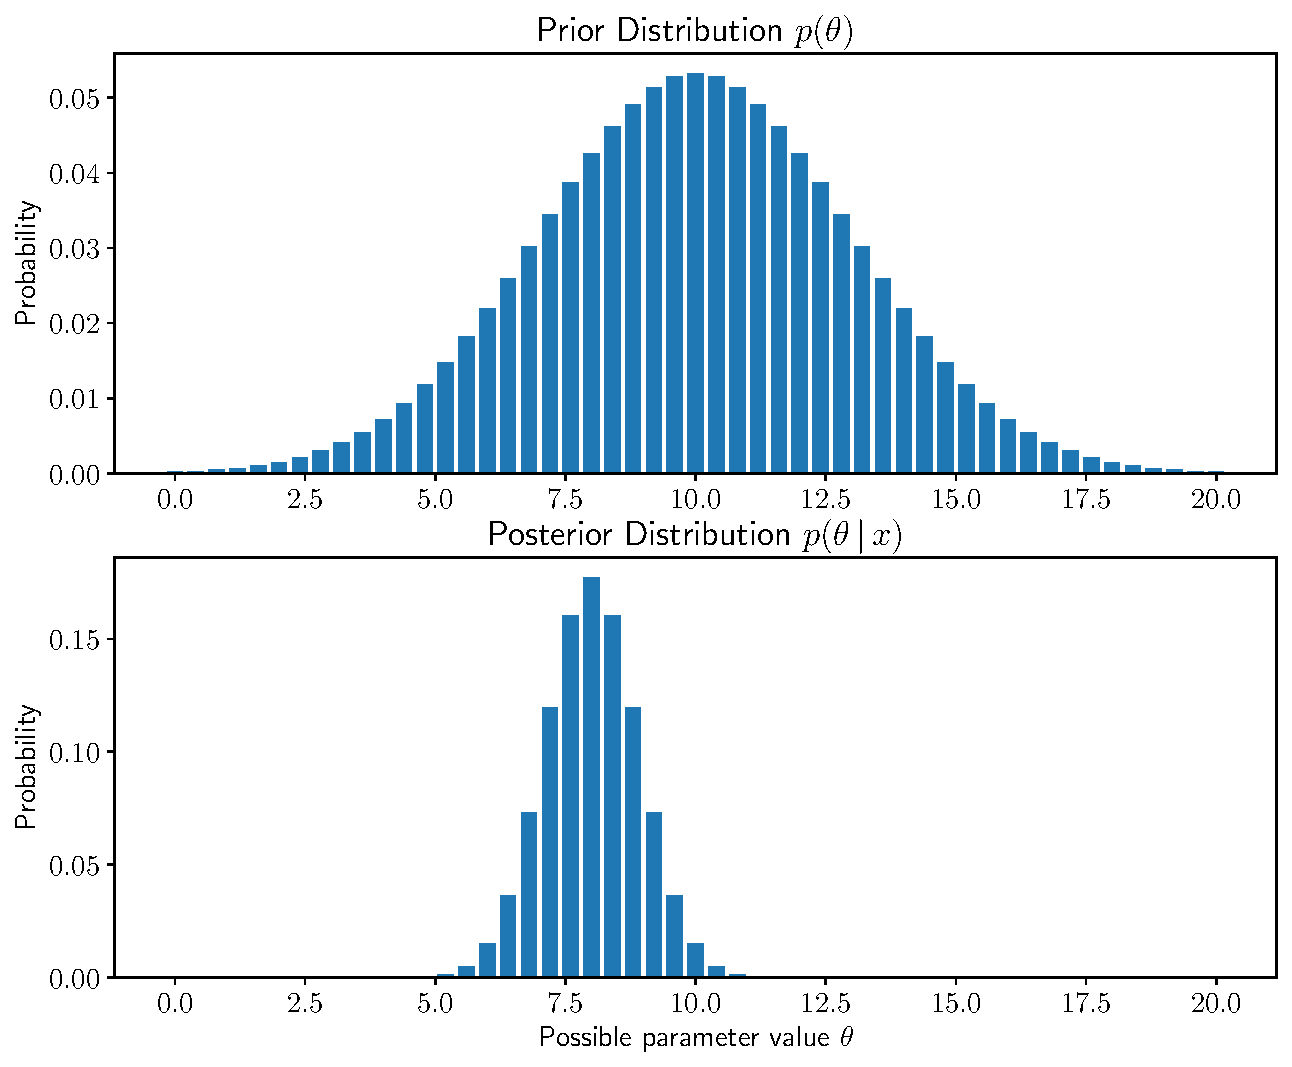
\includegraphics[width=0.5\textwidth]{images/updating.pdf}
\end{center}

\end{frame}


\begin{frame}
\frametitle{Estimating a Proportion}

\begin{itemize}
\item We will now solve the famous problem of estimating a
proportion using a Bayes Box.\pause
\item Suppose there is an election coming up, with two major
parties. 10 people are called to take a poll.\pause
\item Results (data): $\{1, 1, 0, 0, 1, 0, 1, 0, 1, 1\}$\pause
\item What fraction $\theta$ of the entire population supports the party
represented by `1' in the data?
\end{itemize}

\end{frame}

\begin{frame}
\frametitle{Estimating a Proportion --- Uniform Prior}

\centering
{\footnotesize
\begin{tabular}{|c|c|c|c|c|}
\hline
Parameter & Prior & Likelihood & Prior $\times$ Likelihood & Posterior \\
$\theta$  & $p(\theta)$ & $p(x \given \theta)$ & $p(\theta)p(x\given\theta)$ & $p(\theta\given x)$ \\
\hline
0 & 0.0909 & & & \\
0.1 & 0.0909  &  & & \\
0.2 & 0.0909  &  & & \\
0.3 & 0.0909 &  & & \\
0.4 & 0.0909  &  & & \\
0.5 & 0.0909 & & & \\
0.6 & 0.0909 & & & \\
0.7 & 0.0909 & & & \\
0.8 & 0.0909 & & & \\
0.9 & 0.0909 & & & \\
1   & 0.0909 & & & \\
\hline
Total & 1 & & & 1 \\
\hline
\end{tabular}
}

\end{frame}


\begin{frame}[fragile]
\frametitle{Creating the Parameter and Prior Vectors in R}
We will often use R's \mintinline{r}{seq()} and
\mintinline{r}{rep()} functions to do this.\pause

\begin{minted}{r}
theta = seq(0, 1, by=0.1)
prior = rep(1/length(theta), length(theta))
\end{minted}

\end{frame}

\begin{frame}
\frametitle{Likelihood}
We called 10 people and the data was
$\{1, 1, 0, 0, 1, 0, 1, 0, 1, 1\}$. We can reason out the likelihood
--- imagining we know $\theta$, but leaving it as a symbol, so we get
all likelihood values at once.\pause
\begin{align}
P(1 \given \theta) &= \theta \\
P(0 \given \theta) &= 1-\theta \\
P(\{1, 1, 0\} \given \theta) &= \theta\theta(1-\theta) \\
P(\{1, 1, 0, 0, 1, 0, 1, 0, 1, 1\}) &= \theta^6(1-\theta)^4
\end{align}



\end{frame}

\begin{frame}
\frametitle{Likelihood}
In the beginning of this course, finding likelihoods is the hardest
part for many students. Put yourself in the hypothetical situation
of knowing $\theta$ but not knowing the data, and ask yourself
what the probability would be of the data that you got.\\[1em]\pause

Later, this will get easier, when we use
{\bf sampling distributions}
as a stepping stone to getting the likelihood function.

\end{frame}

\begin{frame}[fragile]
\frametitle{Likelihood in R}
We have a formula involving $\theta$, so we can simply use it
in R:

\begin{minted}{r}
lik = theta^6*(1-theta)^4
\end{minted}

\end{frame}

\begin{frame}[fragile]
\frametitle{Solution in R}

\begin{minted}{r}
theta = seq(0, 1, by=0.1)
prior = rep(1/length(theta), length(theta))
lik = theta^6*(1-theta)^4
h = prior*lik
Z = sum(h)
post = h/Z
\end{minted}
\end{frame}


\begin{frame}
\frametitle{Solution --- Plot}

\centering
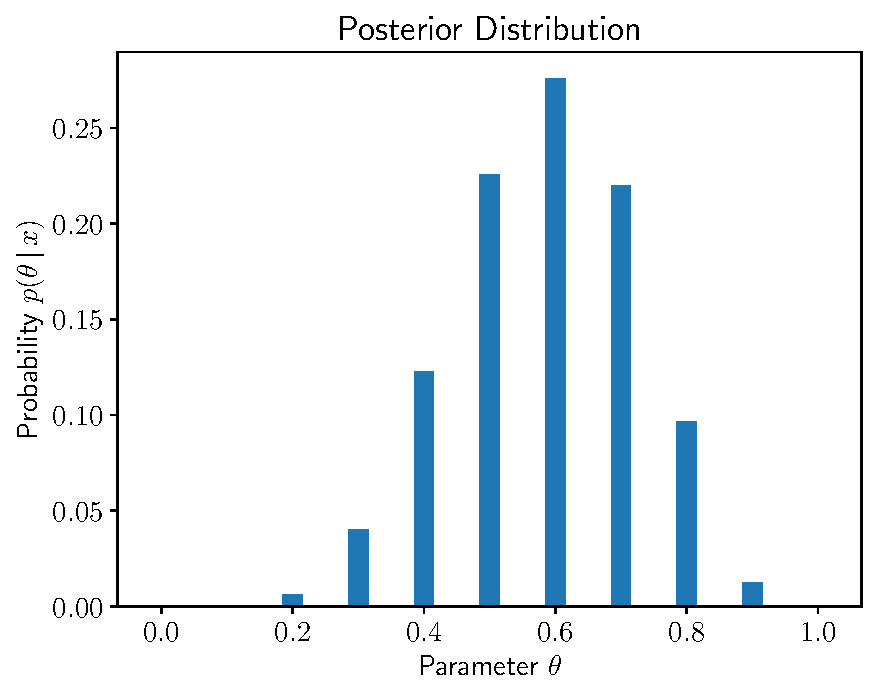
\includegraphics[width=0.7\textwidth]{images/election.pdf}

\end{frame}


\begin{frame}
\frametitle{A Note on Constant Factors in the Likelihood}

\begin{itemize}
\item The bus problem in the notes is very closely related to
this. It uses the binomial distribution as the sampling distribution, from
which we get the likelihood.\pause
\item This is appropriate if you only know about the 6
successes (out of the 10 trials), rather than the full
sequence of successes and failures.\pause
\item The only difference in the formula for the
likelihood is a constant out the front (not involving $\theta$).\pause
\item The likelihoods and marginal likelihood are affected by this constant,
but because we divide by the marginal likelihood, the posterior is the same
whether the constant is there or not.
\end{itemize}

\end{frame}


\begin{frame}
\frametitle{Outputs Again}

\begin{itemize}
\item Recall that the outputs of Bayesian calculations are the posterior distribution
and the marginal likelihood.\pause
\item These --- especially the posterior distribution --- are the complete
answer to the inference problem.
\end{itemize}

\centering

\includegraphics[width=0.3\textwidth]{images/brosh.jpg}

{\tiny (Image credit: Allie Brosh)}

\end{frame}


\begin{frame}
\frametitle{Taxi Problem}

    \begin{columns} % Create two columns
        \column{0.5\textwidth} % Left column (50% width)

        \begin{itemize}
        \item You fall asleep in a foreign city.
        \item When you wake up in the morning, you see a taxi drive by,
              which says {\bf This is taxi number 42}.
        \item How many taxis are in the city?
        \end{itemize}

        \column{0.5\textwidth} % Right column (50% width)
        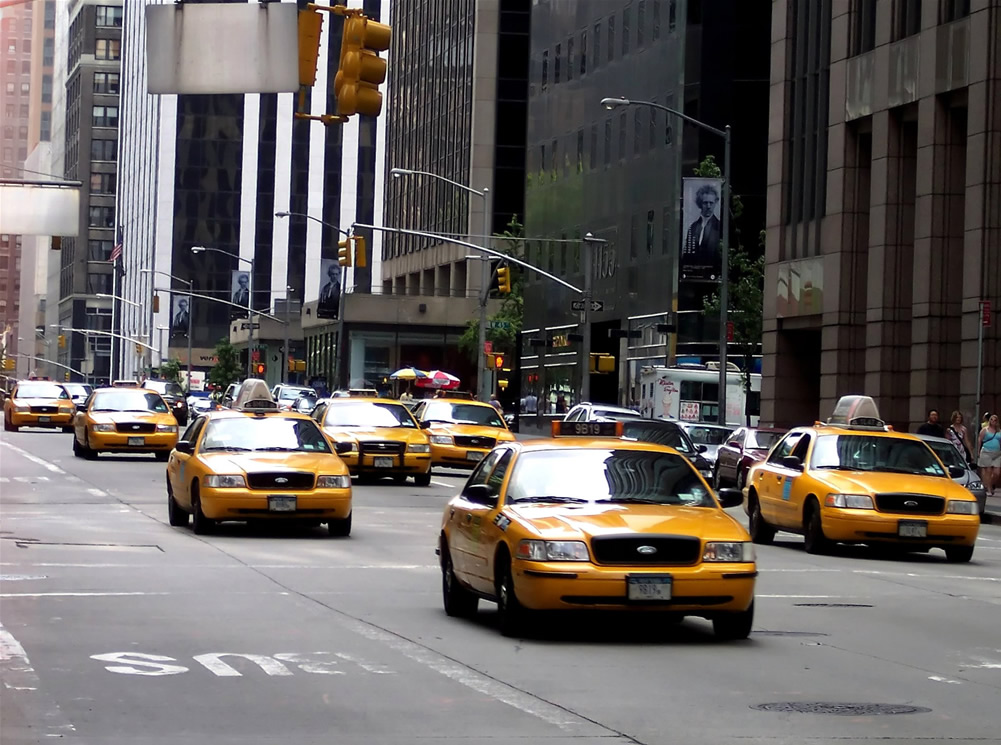
\includegraphics[width=0.95\linewidth]{images/taxis.jpg}
       
         (public domain image)
     \end{columns}

\end{frame}

\begin{frame}
\frametitle{The Parameter and the Data}

\begin{itemize}
\item The unknown parameter, $N$, is the number of taxis in the city.\pause
\item The data, $x$, is the number observed on the taxi that drove past.
\end{itemize}
\pause
Bayes' rule for this circumstance:

\begin{align}
p(N \given x) \propto p(N)p(x \given N)
\end{align}
We have to choose the prior $p(N)$ and the likelihood $p(x \given N)$.

\end{frame}


\begin{frame}
\frametitle{Bayes Box with Uniform Prior}
Let's assume $N \leq 100$ and keep our uniform prior for now.

\centering
{\footnotesize
\begin{tabular}{|c|c|c|c|c|}
\hline
Parameter & Prior & Likelihood & Prior $\times$ Likelihood & Posterior \\
$N$  & $p(N)$ & $p(x \given N)$ & $p(N)p(x\given N)$ & $p(N\given x)$ \\
\hline
1 & 0.01 & & & \\
2 & 0.01  &  & & \\
... &... &... & ...&... \\
41 & 0.01 &  & & \\
42 & 0.01  &  & & \\
43 & 0.01 & & & \\
... &... &... & ...&... \\
99 & 0.01 & & & \\
100   & 0.01 & & & \\
\hline
Total & 1 & & & 1 \\
\hline
\end{tabular}
}

\end{frame}

\begin{frame}
\frametitle{Likelihoods: Direct Reasoning}

\begin{itemize}
\item If $N=1$, with what probability would we observe $x=42$? \pause
\item If $N=41$, with what probability would we observe $x=42$? \pause
\item If $N=42$, with what probability would we observe $x=42$? \pause
\item If $N=100$, with what probability would we observe $x=42$?
\end{itemize}

\end{frame}


\begin{frame}
\frametitle{Likelihoods}

\centering
{\footnotesize
\begin{tabular}{|c|c|c|c|c|}
\hline
Parameter & Prior & Likelihood & Prior $\times$ Likelihood & Posterior \\
$N$  & $p(N)$ & $p(x \given N)$ & $p(N)p(x\given N)$ & $p(N\given x)$ \\
\hline
1 & 0.01 & 0 & & \\
2 & 0.01  & 0  & & \\
... &... &... & ...&... \\
41 & 0.01 & 0 & & \\
42 & 0.01  & 1/42 & & \\
43 & 0.01 & 1/43 & & \\
... &... &... & ...&... \\
99 & 0.01 & 1/99 & & \\
100   & 0.01 & 1/100 & & \\
\hline
Total & 1 & & & 1 \\
\hline
\end{tabular}
}

\end{frame}


\begin{frame}
\frametitle{Likelihoods: from Sampling Distribution}
Imagine we did not know $x$ yet, but we did know $N$, the parameter.
We can assign a probability distribution for $x$ given $N$.
This would be a discrete uniform distribution, and we can write
\begin{align}
x \given N &\sim \textnormal{Uniform}(1, 2, ..., N).
\end{align}\pause

The formula for this probability distribution is
\begin{align}
p(x \given N) &= \left\{
                    \begin{array}{lr}
                    \frac{1}{N}, & x \in \{1, 2, ..., N\} \\
                    0          , & \textnormal{otherwise}.
                    \end{array}
                 \right.
\end{align}
\end{frame}

\begin{frame}
\frametitle{Likelihoods: from Sampling Distribution}
If we take the formula and interpret it as a function of $N$
with $x$ fixed at 42, it reads
\begin{align}
p(x \given N) &= \left\{
                    \begin{array}{lr}
                    \frac{1}{N}, & 42 \in \{1, 2, ..., N\} \\
                    0          , & \textnormal{otherwise}.
                    \end{array}
                 \right.
\end{align}
which is exactly the rule we `guessed' earlier.


\end{frame}

\begin{frame}
\frametitle{Likelihoods: from Sampling Distribution}
In general, we can think of data as being `drawn from'
some distribution\footnote{Philosophically I object, but it is a useful
starting point.}
with unknown parameter $\theta$, written as $p(x \given \theta)$.
This will be a formula involving both $x$ and $\theta$.
\pause

When $x$ is known value (plugged in) but $\theta$ isn't, $p(x \given \theta)$
is now a function of $\theta$ only --- the likelihood function.
You may have seen this in STATS 210 or other courses. If not, this is a
reasonable first place to learn about it.

\end{frame}


\begin{frame}
\frametitle{Likelihoods: from Sampling Distribution}
Since sampling distributions are conditional on $\theta$ but not on the
data $x$, they are kind of a prior but for the data instead of the parameter.

\end{frame}



\begin{frame}[fragile]
\frametitle{Calculating the Posterior in R}
This follows the standard recipe, but the likelihood is slightly trickier
than what we had before.
\begin{minted}{r}
N = seq(1, 100)
prior = rep(1/length(N), length(N))
lik = 1/N
lik[N < 42] = 0
h = prior*lik
Z = sum(h)
post = h/Z
plot(N, post, type="h")
\end{minted}

\end{frame}

\begin{frame}
\frametitle{Taxi Posterior}

\centering
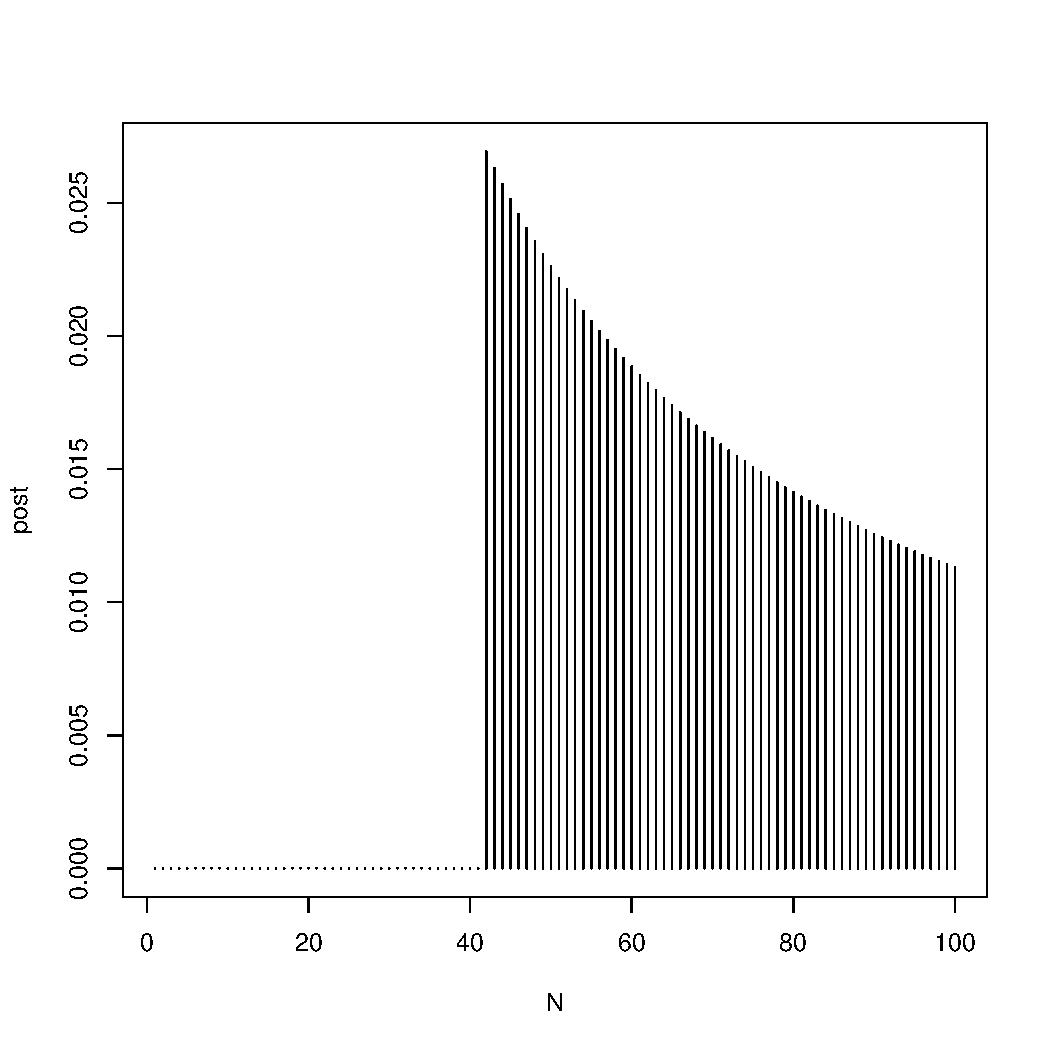
\includegraphics[width=0.6\textwidth]{images/taxi_posterior.pdf}

\end{frame}


\begin{frame}[fragile]
\frametitle{Multiple Data Points}
When the data is more than one number, the likelihood consists
of a product of terms, one for each data point.

Let's analyse the taxi data for three observations
$\{x_1, x_2, x_3\} = \{42, 61, 12\}$.

\end{frame}



\end{document}

